% 80-07(인쇄 80쪽) — 두 스위치 A, B 가 병렬로 놓이고 전구와 직렬로 이어진 회로.
% 스캔 화질이 낮아 TikZ 로 다시 그림(스위치는 경첩점·레버, 전구는 회로 기호로 · 라벨은 원문에 있는 A, B 뿐).
% 스위치가 열린 채로 그려져도 확률은 본문 수치로만 정해지므로 답이 그림에서 읽히지 않는다.
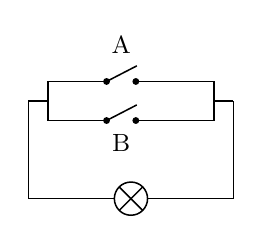
\begin{tikzpicture}[scale=0.62, line width=0.55pt]
  % 바깥 회로: 왼쪽 세로선 → 아래 가로선(전구) → 오른쪽 세로선
  \draw (0.4,2.2) -- (0.4,0.2) -- (2.16,0.2);
  \draw (2.84,0.2) -- (4.6,0.2) -- (4.6,2.2);
  % 바깥 회로와 병렬 블록을 잇는 선
  \draw (0.4,2.2) -- (0.8,2.2);
  \draw (0.8,1.8) -- (0.8,2.6);
  \draw (4.2,2.2) -- (4.6,2.2);
  \draw (4.2,1.8) -- (4.2,2.6);
  % 위 가지 · 스위치 A
  \draw (0.8,2.6) -- (2.0,2.6);
  \draw (2.6,2.6) -- (4.2,2.6);
  \draw (2.0,2.6) -- (2.62,2.92);
  \fill (2.0,2.6) circle (2pt);
  \fill (2.6,2.6) circle (2pt);
  \node[above, font=\small] at (2.3,2.96) {$\mathrm{A}$};
  % 아래 가지 · 스위치 B
  \draw (0.8,1.8) -- (2.0,1.8);
  \draw (2.6,1.8) -- (4.2,1.8);
  \draw (2.0,1.8) -- (2.62,2.12);
  \fill (2.0,1.8) circle (2pt);
  \fill (2.6,1.8) circle (2pt);
  \node[below, font=\small] at (2.3,1.72) {$\mathrm{B}$};
  % 전구
  \draw (2.5,0.2) circle (0.34);
  \draw (2.26,-0.04) -- (2.74,0.44);
  \draw (2.26,0.44) -- (2.74,-0.04);
\end{tikzpicture}
